% !TeX root = ../my-thesis.tex
\chapter{Energieeffizientes Multithreading}

\section{Darstellung der Messwerte}

% Table generated by Excel2LaTeX from sheet 'Tabelle1'
\begin{table}[htbp]
  \centering
  \caption{Laufzeit in Abh\"angigkeit von der Thread Anzahl}
    \begin{tabular}{rrrr}
    \toprule
    \multicolumn{1}{c}{Threads} & \multicolumn{1}{c}{t in ms} & \multicolumn{1}{l}{Speedup} & \multicolumn{1}{l}{Effizienz} \\
    \midrule
    1     & 994358 & 1,000 & 1,000 \\
    \midrule
    2     & 631836 & 1,574 & 0,787 \\
    \midrule
    3     & 507871 & 1,958 & 0,653 \\
    \midrule
    4     & 441615 & 2,252 & 0,563 \\
    \midrule
    5     & 416036 & 2,390 & 0,478 \\
    \midrule
    6     & 387519 & 2,566 & 0,428 \\
    \midrule
    7     & 369424 & 2,692 & 0,385 \\
    \midrule
    8     & 364560 & 2,728 & 0,341 \\
    \midrule
    9     & 364637 & 2,727 & 0,303 \\
    \midrule
    10    & 355893 & 2,794 & 0,279 \\
    \midrule
    11    & 355677 & 2,796 & 0,254 \\
    \midrule
    12    & 364313 & 2,729 & 0,227 \\
    \midrule
    13    & 363055 & 2,739 & 0,211 \\
    \midrule
    14    & 377380 & 2,635 & 0,188 \\
    \midrule
    15    & 383928 & 2,590 & 0,173 \\
    \midrule
    16    & 395553 & 2,514 & 0,157 \\
    \bottomrule
    \end{tabular}%
  \label{tab:Base64Laufzeit}%
\end{table}%


\begin{figure}[H]
	\begin{center}	 
	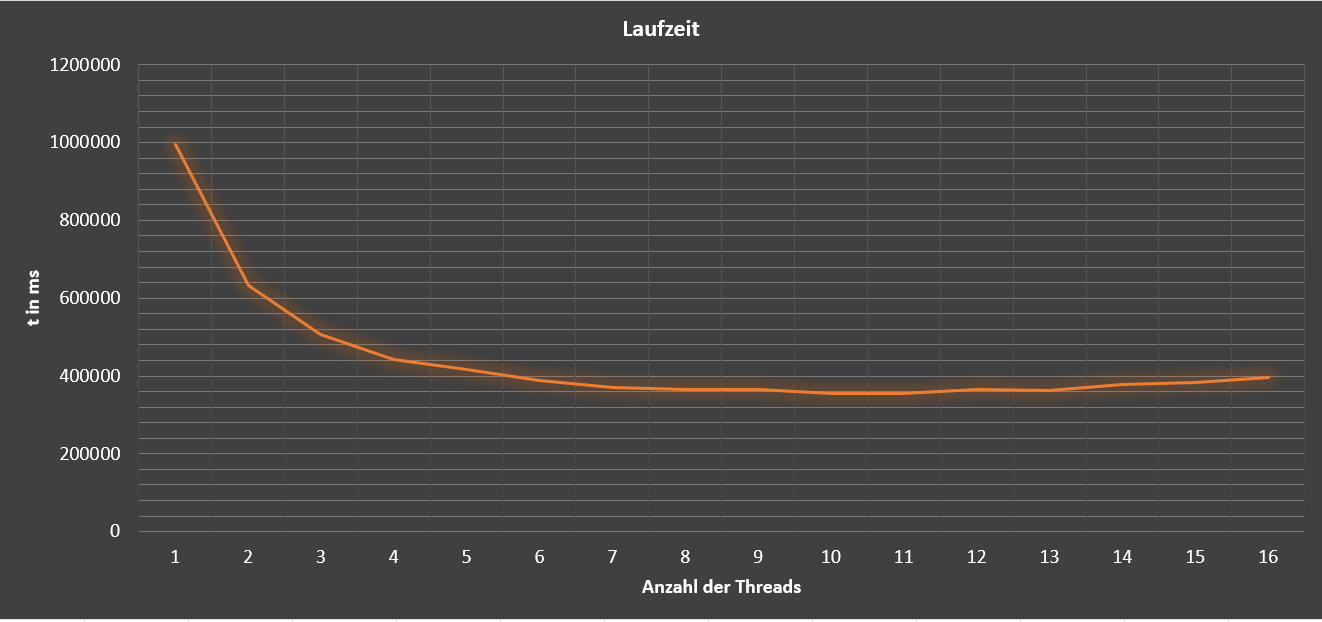
\includegraphics[width=0.8\textwidth]{Base64LaufzeitPic}
	\caption{Laufzeitdiagramm (eigene Abbildung)}
	\label{fig:Base64LaufzeitPic} 
	\end{center}
\end{figure}

% !TeX root = ../my-thesis.tex
% Table generated by Excel2LaTeX from sheet 'Tabelle1'
\begin{table}[htbp]
  \centering
  \caption{durchschnittliche Leistungsaufnahme in Abh\"angigkeit von der Thread Anzahl}
    \begin{tabular}{rrrr}
    \toprule
    \multicolumn{1}{c}{Threads} & \multicolumn{1}{c}{\O U in mV} & \multicolumn{1}{c}{\O I in mA} & \multicolumn{1}{c}{\O P in W} \\
    \midrule
    1     & 4077,382 & 565,944 & 2,306 \\
    \midrule
    2     & 3997,636 & 733,983 & 2,931 \\
    \midrule
    3     & 4029,556 & 860,404 & 3,462 \\
    \midrule
    4     & 4056,719 & 859,178 & 3,479 \\
    \midrule
    5     & 4043,867 & 869,086 & 3,505 \\
    \midrule
    6     & 4028,429 & 900,618 & 3,621 \\
    \midrule
    7     & 4017,545 & 923,407 & 3,705 \\
    \midrule
    8     & 4042,727 & 933,792 & 3,772 \\
    \midrule
    9     & 4063,227 & 901,938 & 3,662 \\
    \midrule
    10    & 4046,045 & 934,489 & 3,775 \\
    \midrule
    11    & 4034,455 & 948,283 & 3,824 \\
    \midrule
    12    & 4074,458 & 856,408 & 3,485 \\
    \midrule
    13    & 4049,000 & 962,385 & 3,486 \\
    \midrule
    14    & 4063,917 & 915,918 & 3,586 \\
    \midrule
    15    & 4021,708 & 926,291 & 3,726 \\
    \midrule
    16    & 4023,542 & 946,001 & 3,806 \\
    \bottomrule
    \end{tabular}%
  \label{tab:Base64Leistung}%
\end{table}%


\begin{figure}[h]
	\begin{center}	 
	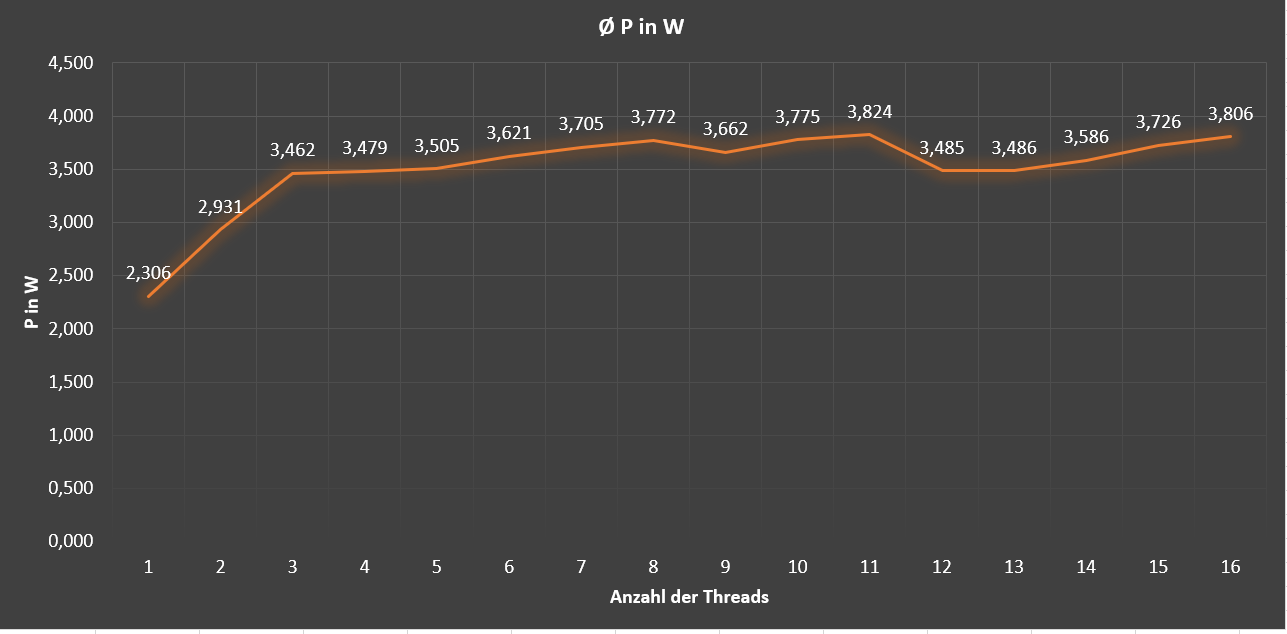
\includegraphics[width=0.8\textwidth]{Base64LeistungPic}
	\caption{durchschnittliche elektrische Leistung in Abhängigkeit von der Thread Anzahl (eigene Abbildung)}
	\label{fig:Base64LeistungPic} 
	\end{center}
\end{figure}

% !TeX root = ../my-thesis.tex
% Table generated by Excel2LaTeX from sheet 'Tabelle1'
\begin{table}[htbp]
  \centering
  \caption{elektrische Arbeit in Abhängigkeit von der Thread Anzahl}
    \begin{tabular}{rr}
    \toprule
    \multicolumn{1}{c}{Threads} & \multicolumn{1}{c}{W in Ws} \\
    \midrule
    1     & 2330,170 \\
    \midrule
    2     & 1891,658 \\
    \midrule
    3     & 1815,574 \\
    \midrule
    4     & 1594,628 \\
    \midrule
    5     & 1532,691 \\
    \midrule
    6     & 1473,056 \\
    \midrule
    7     & 1347,732 \\
    \midrule
    8     & 1296,977 \\
    \midrule
    9     & 1252,836 \\
    \midrule
    10    & 1290,069 \\
    \midrule
    11    & 1306,284 \\
    \midrule
    12    & 1316,109 \\
    \midrule
    13    & 1322,537 \\
    \midrule
    14    & 1374,502 \\
    \midrule
    15    & 1393,833 \\
    \midrule
    16    & 1409,848 \\
    \bottomrule
    \end{tabular}%
  \label{tab:Base64Arbeit}%
\end{table}%


\begin{figure}[H]
	\begin{center}	 
	\includegraphics[width=0.95\textwidth]{Base64LeistungFlächePic}
	\caption{Verlauf der elektrischen Leistung mit einem Thread (eigene Abbildung)}
	\label{fig:Base64LeistungFlächePic} 
	\end{center}
\end{figure}

\begin{figure}[H]
	\begin{center}	 
	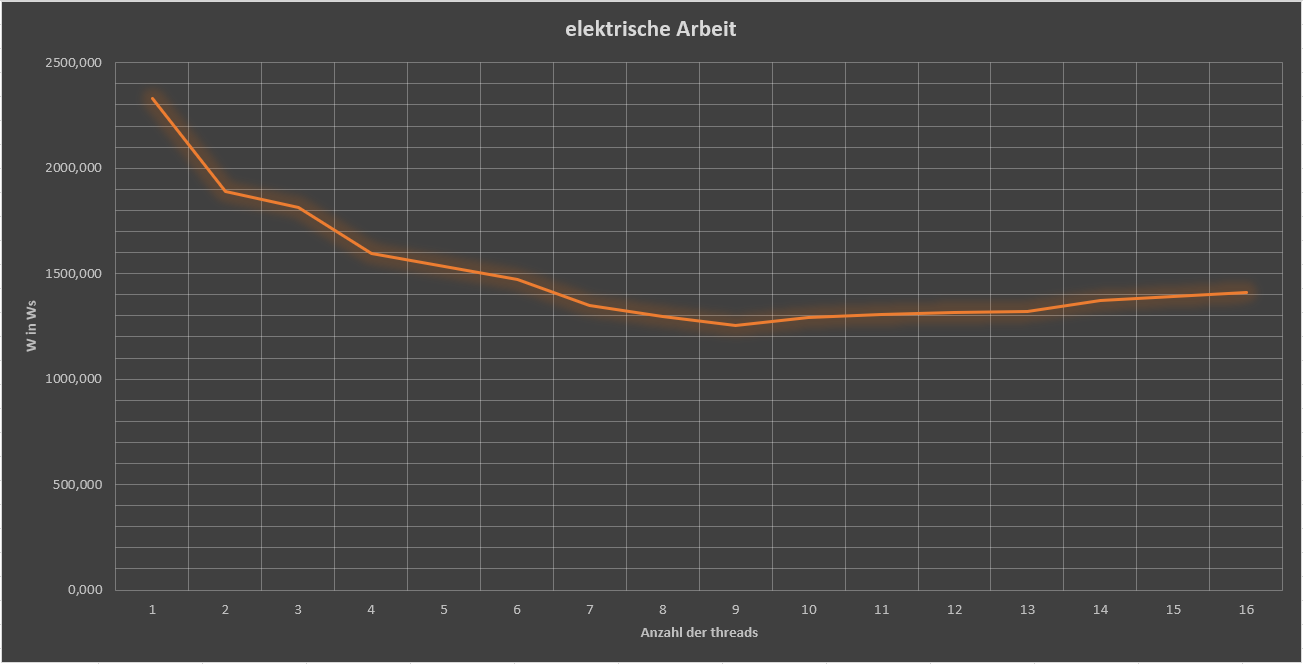
\includegraphics[width=0.95\textwidth]{Base64ArbeitPic}
	\caption{elektrische Arbeit in Abhängigkeit der Thread Anzahl(eigene Abbildung)}
	\label{fig:Base64ArbeitPic} 
	\end{center}
\end{figure}


\section{Auswertung}